% Run on XeLaTeX

\documentclass[12pt, letterpaper]{article}

\usepackage{amsmath}
\usepackage{amsfonts}
\usepackage{graphicx}
\usepackage{multirow}
\usepackage{amssymb}

% set path to images
\graphicspath{{./images/}}

% load persian language and select font
\usepackage{xepersian}
\settextfont{BNazanin}

\title{گزارش کار پروژه اول آنالیز عددی 1}
\author{گروه 6}

\begin{document}
\maketitle

\section{سوال 1}
\subsection{صورت سوال}
فرض کنید \(fl(y)\) عدد \(k\) رقمی قطع شده \(y\) باشد، نشان دهید:

\[\frac{\big| y-fl(y) \big| }{\big| y \big|} \le 10^{-k+1}\]

\subsection{پاسخ}
داریم :

\[  \frac{ \big| 0.d_{1}d_{2}...d_{n} \times{10^n} - 0.d_{1}d_{2}...d_{k} \times{10^n} \big|}{ \big| y \big|}  \]
\[  =   \frac{ \big| 0.000...d_{k+1}d_{k+2}...d_{n} \times{10^n}\big|}{ \big| y \big|}  \]
\[  =   \frac{ \big| 0.d_{k+1}d_{k+2}...d_{n-k} \times{10^{n-k}}\big|}{ \big| y \big|}  \]
\[  =   \frac{ \big| 0.d_{k+1}d_{k+2}...d_{n-k} \times{10^{n-k}}\big|}{ \big| 0.d_{1}d_{2}...d_{n} \times{10^n} \big|}  \]
\[  =   \frac{ \big| 0.d_{k+1}d_{k+2}...d_{n-k} \times{10^{-k}}\big|}{ \big| 0.d_{1}d_{2}...d_{n} \big|}  \]

مخرج را تا یک رقم اعشار قطع میکنیم. داریم:
\[ 0.d_{1} \le 0.d_{1}d_{2}... \le 1\]
پس:
\[  = \frac{ \big| 0.d_{k+1}d_{k+2}...d_{n-k} \times{10^{-k}}\big|}{ 0.d_{1}}  \]
\[  = \frac{ \big| 0.d_{k+1}d_{k+2}...d_{n-k} \times{10^{-k}}\big|}{ d_{1} \times 0.1}  \]
\[  = \frac{ \big| 0.d_{k+1}d_{k+2}...d_{n-k}\big|}{ d_{1}} \times \frac{10^{-k}}{\frac{1}{10}}  \]
\[  = \frac{ \big| 0.d_{k+1}d_{k+2}...d_{n-k}\big|}{ d_{1}} \times 10^{-k+1}  \]
چون که:
\[0 < 0.d_{k+1}d_{k+2}...d_{n-k} < 1\]
\[ 1 \le d_{1} \le 9\]
\[0 < \frac{ 0.d_{k+1}d_{k+2}...d_{n-k}}{d_{1}} < 1\]
پس
\[  = \frac{ \big| 0.d_{k+1}d_{k+2}...d_{n-k}\big|}{ d_{1}} \times 10^{-k+1}  \le 10^{-k+1} \]
$\blacksquare$



% leave space between question 1 and 2
\vspace{5mm}

% start of question 2
\section{سوال 2}
\subsection{صورت سوال}
فرض کنید
\(f(x) = \frac{2 \cdot log(1+x) \: + \: 2 \cdot i tan^{-1}(ix) \: + \: x^2}{-x^4}\)
و 
\(\lim_{x\to 0}\frac{f(x)}{x^p} = C \ne 0\)
با داشتن سری مکلورن توابع 
\(log(x)\)
و 
\(tan^{-1}(x)\)
مقادیر 
\(C\)
و 
\(p\)
را بیابید.

\subsection{پاسخ}
همانطور که در فایل میپل حل این سوال قابل مشاهده است، در مرحله اول با تعریف ظابطه اصلی تابع و رسم نمودار آن سعی میکنیم درکی هندسی از رفتار آن بیابیم. نمودار اول نشان میدهد که تابع در 0 به مقداری نزدیک به 0 میل میکند. اما با برسی دقیق تر و محدود کردن دامنه نمایش نمودار مشاهده میشود که تابع در مقادیر نزدیک به صفر شدیدا نوسان میکند. \\
% insert the 2 plot of f(x) 

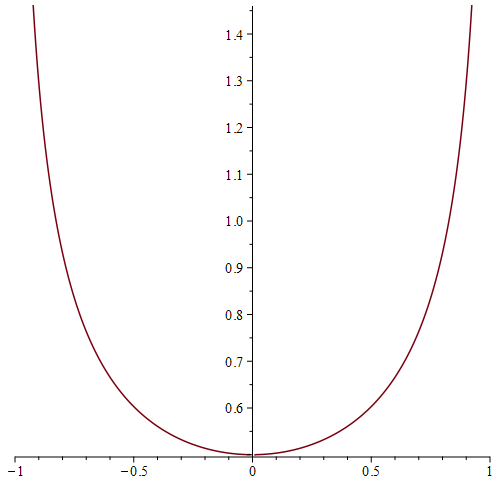
\includegraphics[height=5cm, width=7cm]{figure1.png}
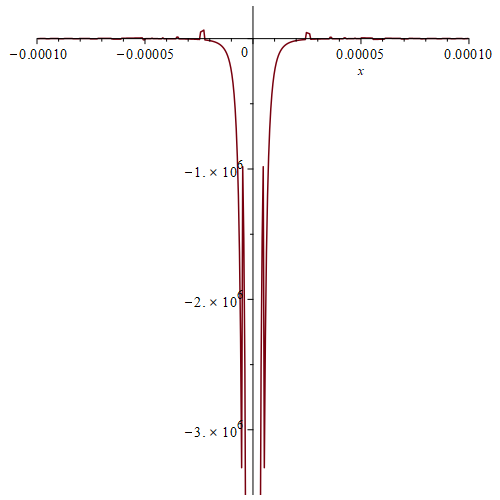
\includegraphics[height=5cm, width=7cm]{figure2.png}
\\


برای حل سوال در ابتدا بسط مکلورن توابع را تا درجه 10 محاسبه میکنیم. نرم افزار میپل از
\(O(x^y)\)
 برای نمایش درجه خطا در یک سری تیلور استفاده میکند. یا این توصیف با افزایش تعداد جملات سری تیلور یا درجه آن میتوان خطا را تا حد توانایی مجاسباتی کامپیوتر کاهش داد. اما چون در این مورد 
\(x\)
 بسیار نزدیک به 0 است میتوان با همین درجه پیش رفت چرا که وقتی 
\(x\) 
 نزدیک به صفر است 
\(x^{11}\)
 بسیار کوچک خواهد بود.
\\
\(Order=20\)
برای این است که میپل سری هارا تا درجه حداکثر 20 محاسبه کند و خطا کمی بیشتر کاهش پیدا کند. همانطور که گفته شد جملات
\(O(21)\)
و 
\(O(20)\)
را از سری ها حذف میکنیم. تابع 
\(f_2(x)\)
 را با چندجمله ای ها تعریف میکنیم. تابعی به صورت زیر تعریف میکنیم:
\[Lim(n) = \lim_{x\to 0}\frac {f_2(x)}{x^n}\]

\vspace{5 mm}
مقادیر 
\(Lim\)
 را برای 
\(n\)
 از 1 تا 10 محاسبه میکنیم و همانطور که مشاهده میشود بخشی از حدود تعریف نشده است.
تابع \(Lim\) را این بار با اعمال قاعده هوپیتال تعریف میکنیم و دوباره مقادیر \(Lim\) را برای \(n\) از 1 تا 10 محاسبه میکنیم. میبینیم که
\[ \lim_{x\to 0}\frac {f_2(x)}{x^2} = \frac{1}{3}\]
پس 
\[ L = \frac{1}{3}, \: p = 2\]


\section{سوال 3}
\subsection{صورت سوال}
با استفاده از یک برنامه عددی و تعریف دنباله ای سری ها نشان دهید سری های زیر به ترتیب همگرا و واگرا هستند.
\[ \sum_{i=1}^{\infty} \frac {1}{n^2}\]
\[ \sum_{i=1}^{\infty} \frac {1}{n}\]



\subsection{پاسخ}
% add logical expressions as description of answer

طبق تعریف همگرایی دنباله ها داریم:
\[\exists \! \alpha\! \in\! \mathbb{R} \quad \forall \varepsilon \! > \! 0 \quad \exists N\! > \! 0 \quad \forall n\! >\! N\quad ; \quad \big| \alpha_{n} - \alpha \big|\! <\! \varepsilon \]
در صورت صدق گزاره بالا گوییم دنباله 
\((\alpha_{n})\)
به 
$\alpha$
همگراست. گوییم دنباله ای واگراست اگر همگرا نباشد. پس نقیض منطقی گزاره بالا را محاسبه میکنیم:
\[\forall \! \alpha\! \in\! \mathbb{R} \quad \exists \varepsilon \! > \! 0 \quad \forall N\! > \! 0 \quad \exists n\! >\! N\quad ; \quad \big| \alpha_{n} - \alpha \big|\! \ge\! \varepsilon \]
با این توصیف الگوریتم را به این صورت می سازیم تا با گرفتن 
$\alpha$
 و 
$N$
به عنوان ورودی به دنبال کمترین میزان 
$\varepsilon$
 بگردد و به همراه اندیس عضو دنباله برگرداند. این الگوریتم هم برای نشان دادن همگرایی و هم واگرایی قابل استفاده است.
\\
فایل متلب 
$Sequence.m$
تعریف دنباله است که میتوان با تغییری کوچک دنباله 
$\frac{1}{n}$
را به 
$\frac{1}{n^2}$
 تبدیل کرد و برعکس. 
$Convergence.m$
فایل الگوریتم است که تابعی است در متلب که با گرفتن 
$\alpha$ 
 و 
$N$
مقادیر خواسته شده را برمیگرداند.
$main.m$
 فایل اجرایی است که مقادیر رندوم برای 
$\alpha$
 انتخاب میکند و با اجرای الگوریتم مقادیر را گرفته و در یک آرایه ذخیره میکند.
\\
 فایل های 
$.mat$
در پوشه 
$MATLAB$
 ارایه های ذخیره شده برای اجرای های مختلف اند. پیشوند 
$C$
 نمایش دهنده دنباله 
$\frac{1}{n}$ و $D$
نمایش دهنده
 $\frac{1}{n^2}$ 
است. 
\\
برای اثبات همگرایی دنباله ، طبق تعریف انتظار داریم برای هر مقدار 
$\alpha$ 
ای یا یک $n$ 
با $\varepsilon$
 کوچک پیدا شود یا
 $n$ 
بزرگی پیدا شود. شکل های زیر جدول مربوط به آرایه اجراهای مجزا از الگوریتم برای مقادیر رندوم 
$\alpha$
 اند.
\\
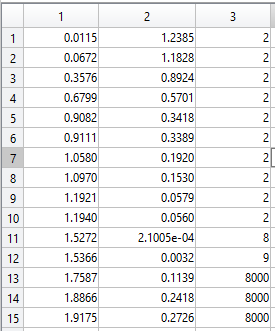
\includegraphics[height=10cm, width=75mm]{figure3.png}
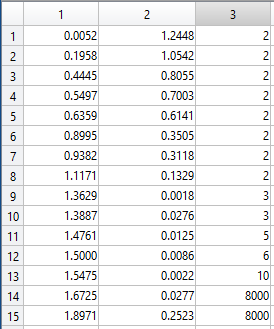
\includegraphics[height=10cm, width=75mm]{figure4.png}
\vspace{10mm}
\\
ستون اول مقادیر 
$\alpha$ 
ستون دوم مقادیر 
$\varepsilon$ 
و ستون سوم مقادیر 
$n$ 
است. همانطور که قابل مشاهده است برای مقادیری از 
$\alpha$ $n$ 
کوچک است و به صورت ناگهان مقادیر 
$n$
 به
 $8000$ 
میرود که حد محاسبه اعضای دنباله است. این به این معنی است که دنباله همگرا به مقداری میان این دو 
$\alpha$
 است.
\\
برای اثبات واگرایی انتظار داریم برای هر 
$\alpha$
یک 
$n$
کوچک و یک 
$\varepsilon$
 کوچک پیدا شود.


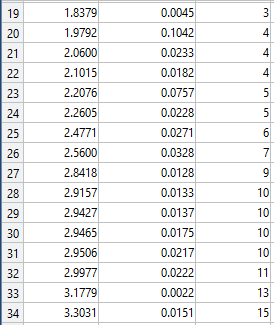
\includegraphics[height=10cm, width=75mm]{figure5.png}
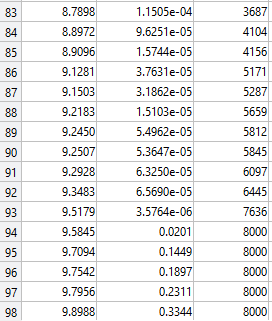
\includegraphics[height=10cm, width=75mm]{figure6.png}

\vspace{10mm}
فایل های 
$ D-ARR5.mat , C-ARR.mat $
شامل داده های بسیار بزرگ تری نسبت به موارد ذکر شده در گزارش هستند اما همچنان ادعای مطرح شده را  تصدیق میکنند.
\vspace{10mm}
\\

\end{document}























